\documentclass[xcolor=dvipsnames]{beamer}
\usepackage[english]{babel}
\usepackage[latin1]{inputenc}
\usepackage{times}
\usepackage[T1]{fontenc}
\usepackage{graphicx}
\usepackage[absolute, overlay]{textpos}
\usepackage{tikz}
\usepackage{multimedia}
\usepackage{soul}
\usepackage{cancel}
\def\urltilda{\kern -.15em\lower .7ex\hbox{\~{}}\kern .04em}
\def\deg{^{\circ}}

\setlength{\TPHorizModule}{0.01\textwidth}
\setlength{\TPVertModule}{\TPHorizModule}
\definecolor{darkyellow}{rgb}{1,0.75,0}
\definecolor{black}{rgb}{0,0,0}
\definecolor{skyblue}{rgb}{0.7,0.8,1.0}
\definecolor{black}{rgb}{0,0,0}
\definecolor{darkgrey}{rgb}{0.3,0.3,0.3}
\definecolor{medgrey}{rgb}{0.5,0.5,0.5}
\definecolor{lightgrey}{rgb}{0.8,0.8,0.8}
\definecolor{lightMahogany}{rgb}{0.9,0.8,0.8}
\definecolor{darkMahogany}{rgb}{0.5,0.2,0.2}
\definecolor{darkgreen}{rgb}{0,0.7,0}
\definecolor{orange}{rgb}{0.8,0.5,0.1}

\newcommand{\manual}[1]{
  \begin{tikzpicture}[x=\textwidth, y=0.82\textheight]%, >=angle 90]
    \useasboundingbox (0, 0) rectangle (1, 1);
    #1
  \end{tikzpicture}
}

%%% Custom nodes.

\newcommand{\basenode}[4]{
  \node[outer sep=6pt, anchor=#3] (#1) at (#2){#4};
}

\newcommand{\emptynode}[2]{
  \basenode{#1}{#2}{base}{}

}

\newcommand{\minipagenode}[5]{
  \basenode{#1}{#2}{#3}{
    \begin{minipage}{#4}
      \vspace*{-12pt}
      {#5}
      \vspace*{-8pt}
  \end{minipage}}

}

\newcommand{\imagenode}[5]{
  \minipagenode{#1}{#2}{#3}{#4}{%
    \includegraphics[width=\textwidth]{#5}%
  }
}

%%% Connectors.

\newcommand{\connect}[4]{%
  \draw[<->, color=darkpurple, line width=1pt, out=#3, in=#4] (#1) to (#2);
}
\newcommand{\connectcolor}[5]{%
  \draw[<->, color=#5, line width=1pt, out=#3, in=#4] (#1) to (#2);
}
\newcommand{\hconnect}[3]{%
  \draw[<->, color=darkpurple, line width=1pt]
  (#1.east) .. controls +(right:#3) and +(left:#3) .. (#2.west);
}
\newcommand{\vconnect}[3]{%
  \draw[<->, color=darkpurple, line width=1pt]
  (#1.south) .. controls +(down:#3) and +(up:#3) .. (#2.north);
}

\newcommand{\src}[2]{%
  {
    \footnotesize
    \href
    {https://gambit.hepforge.org/trac/browser/modules/#1}
    {\textcolor{darkMahogany}{\texttt{#2}}}
  }
}

\newenvironment{litemize}
{\usebeamercolor[fg]{item color}%
\scriptsize\begin{list}{$\bullet$}{%
\setlength{\itemindent}{0pt}%
\setlength{\labelwidth}{10pt}%
\setlength{\leftmargin}{15pt}%
}}
{\end{list}}


\mode<presentation>
{
  \usetheme{Warsaw}
  \usecolortheme[named=Mahogany]{structure}	
  \setbeamercovered{transparent}
  \setbeamercolor*{section in toc}{bg=white, fg=Mahogany}
}

%\beamerdefaultoverlayspecification{<+->}

\AtBeginSubsection[]
{
  \begin{frame}<beamer>
    \frametitle{Outline}
  \begin{columns}[t]
	\column{0.8\textwidth}
	\tableofcontents[sections={1-3}, currentsection, currentsubsection]
  \end{columns}	
  \end{frame}
}

\setbeamertemplate{subsection in head/foot shaded}
{\textcolor{structure!70!white}{\insertsubsectionhead}}
\setbeamertemplate{subsection in head/foot}{\textcolor{white}\insertsubsectionhead}

\title[{\textcolor{white}GAMBIT Core + Model News}]{\textcolor{white}{GAMBIT Core + Model News}}
\author[\textcolor{medgrey}{Pat Scott -- Mar 24 -- GAMBIT III, Adelaide}]{Pat Scott}
\institute{\small{McGill/Imperial}}
\date[Oct 8 2012]{Slides available from Workshop Indico page}
\pgfdeclareimage[height=1.5cm]{gambit-logo}{Logo_Final}
\logo{\pgfuseimage{gambit-logo}}

\subject{Talks}

\begin{document}

\begin{frame}
  \titlepage
\end{frame}


\begin{frame}
\frametitle{Status at Gambit II: CoreChain example}
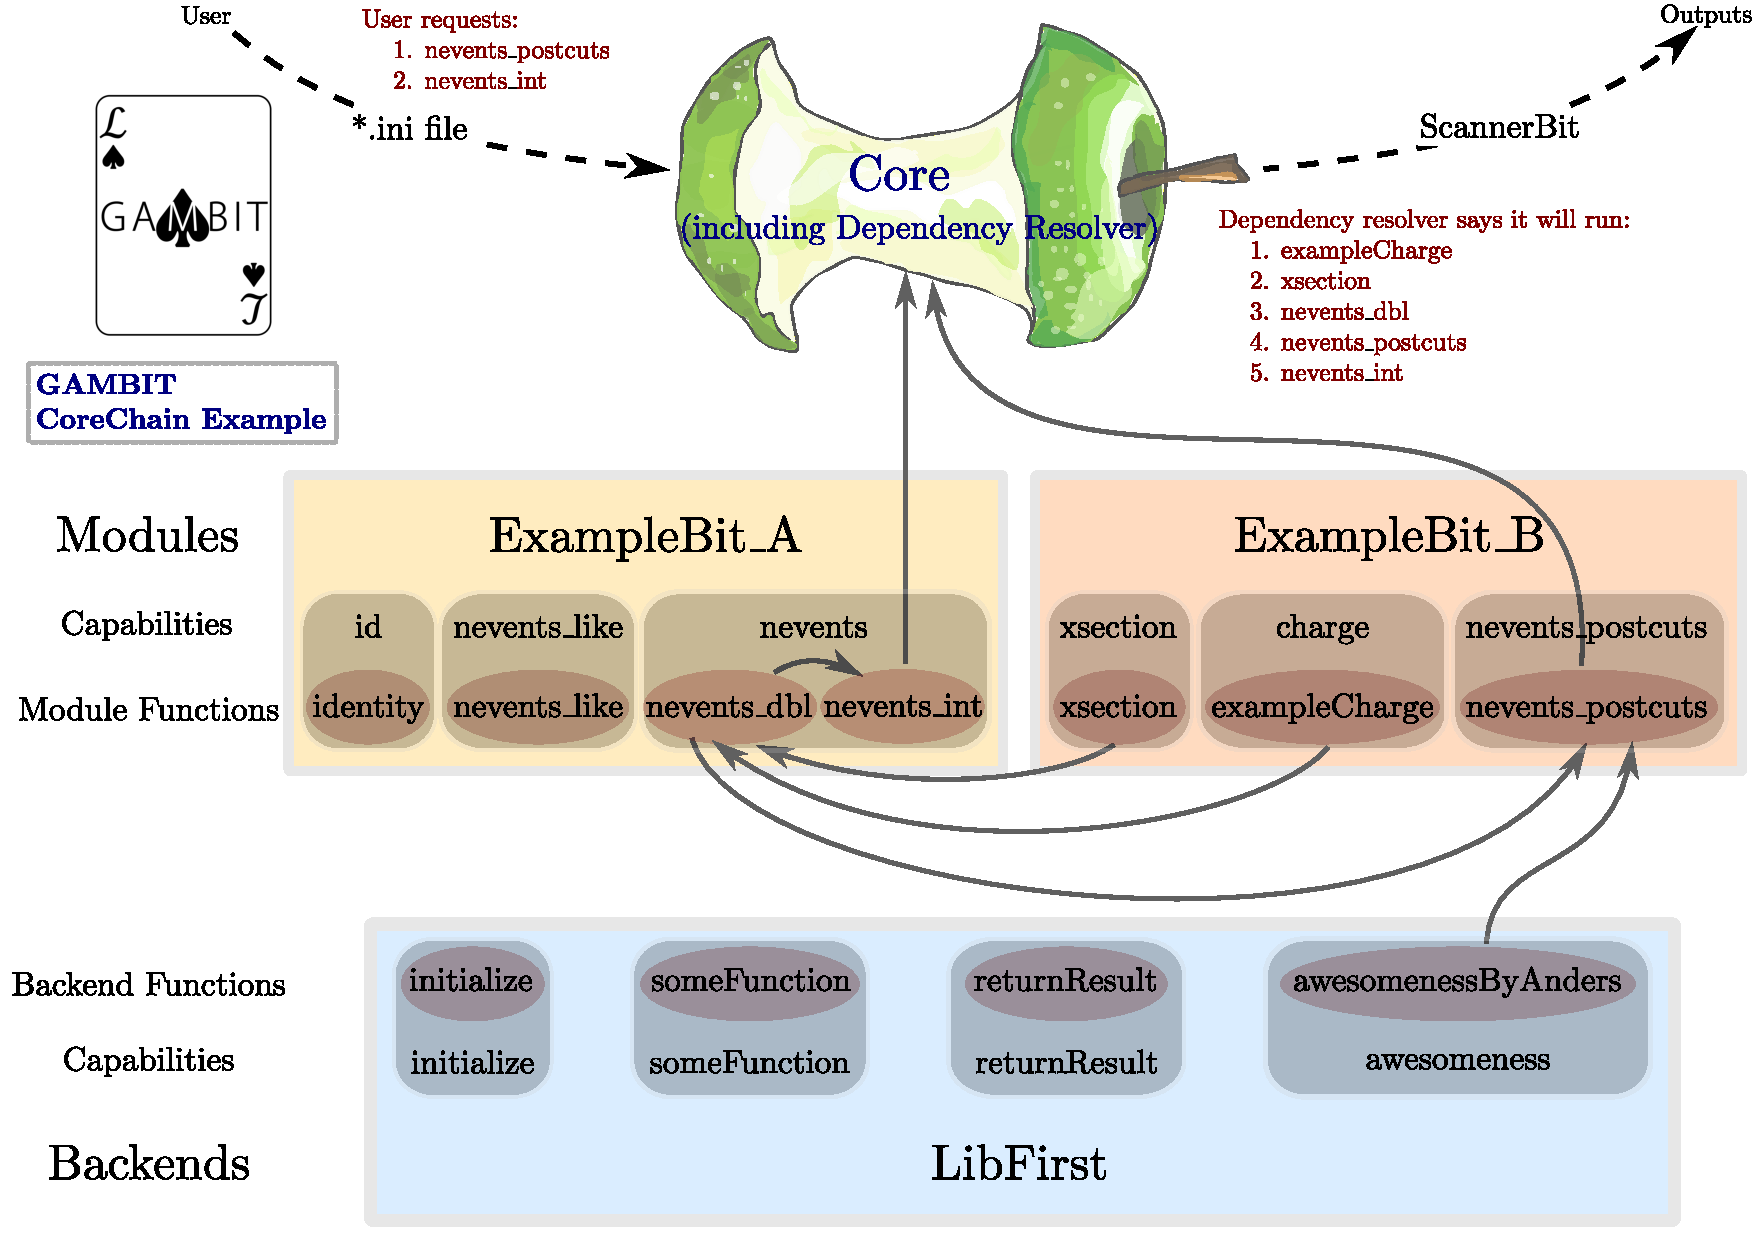
\includegraphics[width=\linewidth]{coreChainDiagram_example_wlogo}
\end{frame}


\begin{frame}
\frametitle{Major updates since Stockholm}

\begin{itemize}

\item Pipes
\item Backend extensions
\item Parallelised module function evaluation with OpenMP `rollcall loops' 
\item Rollcall extensions
\begin{itemize}
  \item Module initialisation functions
  \item Conditional backend requirements
  \item Error-control in rollcall macros 
\end{itemize}
\item Module standalone compilation 
\item Gambit type-inclusion scheme
\item 3 $\times$ main examples
\item Errors, logs, names, etc

\end{itemize}


\end{frame}


\begin{frame}
\frametitle{Pipes}

\begin{itemize}
\item No more macro calls from within module functions \\$\rightarrow$ \texttt{Pipes::$function\_name$::$x$}
\item Safe pointers instead to all the GAMBIT things a function might care about. \alert{These are the only ways in+out!!}\vspace{3mm}
\item Here $x =$\begin{itemize}
\item \texttt{Dep::$dependency\_capability$}  Declared dependencies
\item \texttt{BEReq::$backend\_requirement\_capability$}  Declared backend requirements
\item \texttt{Models}  Current models (only ones this function is allowed to work with)
\item \texttt{runOptions}  Options passed in from the ini file
\item \texttt{Loop::$stuff$} Loop tools (more later)
\end{itemize}\vspace{3mm}
\item Examples:\begin{itemize}
\item \src{ExampleBit_A/src/ExampleBit_A.cpp}{ExampleBit\_A/src/ExampleBit\_A.cpp}
\item \src{ExampleBit_B/src/ExampleBit_B.cpp}{ExampleBit\_B/src/ExampleBit\_B.cpp}
\end{itemize}
\end{itemize}

\end{frame}


\begin{frame}
\frametitle{Parallelised module function evaluation with OpenMP `rollcall loops'} 

Thread-safe OpenMP parallelised loops over module functions\vspace{3mm}

\src{ExampleBit_A/include/ExampleBit_A_rollcall.hpp}{ExampleBit\_A/include/ExampleBit\_A\_rollcall.hpp}\\
\src{ExampleBit_A/src/ExampleBit_A.cpp}{ExampleBit\_A/src/ExampleBit\_A.cpp}

\begin{itemize}
\item \texttt{Loop::executeIteration($it$)} Run iteration number $it$ of the loop (from Loop Manager)
\item \texttt{Loop::iteration} Current loop iteration number (in Nested Function)
\end{itemize}

\vspace{4mm}
The following should be obvious, but in case not:
\begin{itemize}
\item Any module functions put inside a loop must be threadsafe themselves
\item Any calls to backends must be to threadsafe backend functions
\end{itemize}

\end{frame}


\begin{frame}
\frametitle{Rollcall extensions}

\begin{itemize}
  \item Module initialisation functions
    \src{ExampleBit_B/src/ExampleBit_B.cpp}{ExampleBit\_B/src/ExampleBit\_B.cpp}
  \item Conditional backend requirements
    \src{ExampleBit_B/include/ExampleBit_B_rollcall.hpp}{ExampleBit\_B/include/ExampleBit\_B\_rollcall.hpp}\\
  \item Error-control in rollcall macros 
  \item \alert{Proposed:} compact and/or argument-aware backend req declarations (during the week)
\end{itemize}

\end{frame}


\begin{frame}
\frametitle{Backend extensions}

\begin{itemize}
\item Common block / struct access now happens entirely by pointers (BE\_VARIABLE)\\
  \src{Backends/include/backend_libfirst.hpp}{Backends/include/backend\_libfirst.hpp}
  \src{ExampleBit_B/src/ExampleBit_B.cpp}{ExampleBit\_B/src/ExampleBit\_B.cpp}
\item Elegant optional array reindexing scheme for Fortran arrays implemented (Farrays; Lars)
  \src{Backends/lib/libFarrayTest.f90}{Backends/lib/libFarrayTest.f90}
  \src{Backends/include/backend_libFarrayTest.hpp}{Backends/include/backend\_libFarrayTest.hpp}
  \src{ExampleBit_A/src/ExampleBit_A.cpp}{ExampleBit\_A/src/ExampleBit\_A.cpp}
\item The BOSS is coming\ldots (Anders)
\end{itemize}

\end{frame}


\begin{frame}

\frametitle{Module standalone complilaton}

\begin{itemize}
\item Fully standalone compilation of GAMBIT physics modules now possible
\item Requires inclusion of\src{Utils/include/standalone.hpp}{Utils/include/standalone.hpp} and \texttt{\footnotesize$MODULE$/include/$MODULE$\_rollcall.hpp} from main file
\item All modules must ship \alert{with}: Models, Backends, Utils, Logs, Printers, contrib
\item All modules must ship \alert{without}: Core, other modules (incl. ScannerBit)
\item Type inclusion headers will need to be (re-)written by Python scripts for ease of use
\end{itemize}
\src{ExampleBit_A/examples/ExampleBit_A_standalone_example.cpp}{ExampleBit\_A/examples/ExampleBit\_A\_standalone\_example.cpp}

\end{frame}


\begin{frame}

\frametitle{Gambit type-inclusion scheme}

\begin{itemize}
\item \textbf{Common return types:}\\ in \src{Utils/include/shared_types.hpp}{Utils/include/shared\_types.hpp}
\item \textbf{Module-specific types:}\\ in \texttt{\footnotesize $MODULE$/include/$MODULE$\_types.hpp}, then included in \src{Utils/include/types_rollcall.hpp}{Utils/include/types\_rollcall.hpp}
\item \textbf{Model-specific types:}\\ in \texttt{\footnotesize Models/models/$MODEL$\_types.hpp}, then included in \src{Utils/include/types_rollcall.hpp}{Utils/include/types\_rollcall.hpp}
\item \textbf{Backend-specific types:}\\ in \texttt{\footnotesize Backends/include/$BACKEND$\_types.hpp}, then included in \src{Utils/include/shared_types.hpp}{Utils/include/shared\_types.hpp}
\end{itemize}
\begin{columns}
\column{0.96\textwidth}
Eventually, inclusion of module, model and backend-specific type headers into \texttt{\footnotesize shared\_types.hpp} and \texttt{\footnotesize types\_rollcall.hpp} will happen automagically in the harvester script 
\column{0.05\textwidth}
\end{columns}

\end{frame}


\begin{frame}

\frametitle{3 $\times$ main examples}

\begin{itemize}
\item sandbox: \src{Core/examples/gambit_example.cpp}{Core/examples/gambit\_example.cpp}
\item minimal: \src{Core/examples/gambit_example_minimal.cpp}{Core/examples/gambit\_example\_minimal.cpp}
\item standalone: \src{ExampleBit_A/examples/ExampleBit_A_standalone_example.cpp}{ExampleBit\_A/examples/ExampleBit\_A\_standalone\_example.cpp}
\item Makefile structure currently consists of \src{makefile.common}{makefile.common} called by compiler-specific \texttt{\footnotesize makefile.$my\_compiler$} 
\end{itemize}

\end{frame}


\begin{frame}

\frametitle{Errors, logs, names, etc}
\begin{itemize}
\item Naming convention changed GAMBIT$\rightarrow$Gambit in all files (\texttt{namespace Gambit})
\item Logs, Models, Backends, Printers, Utils, (Priors?)
\item Proper exception handling system implemented -- \alert{Use it!}\\
\item Proper logging system implemented -- \alert{Use it!}
\end{itemize}
\src{Utils/src/error_handlers.cpp}{Utils/src/error\_handlers.cpp}\\
\src{ExampleBit_B/src/ExampleBit_B.cpp}{ExampleBit\_B/src/ExampleBit\_B.cpp}\\
\src{gambit.yaml}{gambit.yaml}

\end{frame}



\end{document}

